\documentclass[12pt letter]{report}
\input{./template/preamble}
\input{./template/macros}
\input{./template/letterfonts}

\title{\Huge{Basic Structures: Sets, Functions, Sequences, Sums, and Matrices}}
\author{\huge{Madiba Hudson-Quansah}}
\date{}
\usepackage{parskip}
\usepackage{parskip}
\usepackage{proof}
\setcounter{tocdepth}{4}
\setcounter{secnumdepth}{4}


\begin{document}
\maketitle
\newpage
\pdfbookmark[section]{\contentsname}{too}
\tableofcontents
\pagebreak

\chapter{Sets}

\dfn{Set}{
	An unordered collection of objects, called \textit{elements} or \textit{members} of the set. A set contains elements
	and, we can denote this as  $a \in A$ where $a$ is an element of the set $A$, or $a \notin A$, where $a$ is not an
	element of the set $A$.
}

There are several ways to describe a set:
\begin{description}
	\item[Roster notation] $\left\{ 1, 2, 3, 4, 5 \right\} $
	\item [Set-Builder notation] Where all the elements of a set are described by a property they satisfy.i.e. The set $O$ of
	      all odd positive numbers less than 10 can be expressed as $ O =  \left\{ x  \mid  x \text{ is an odd positive
			      integer less than } 10  \right\}  $ or specifying the domain of discourse, $O =  \left\{ x \in \mathbb{Z}^{+}
		      \mid x \text{ is odd and } x < 10 \right\} $, or the set of all positive rational numbers $\mathbb{Q}^{+}$
	      can be expressed as $\mathbb{Q}^{+} = \left\{ x \in \mathbb{R}  \mid x = \frac{p}{q}
		      \text{, for some positive integers $q$ and $p$}\right\}  $
\end{description}

\dfn{Equality of Sets}{
	Two sets $A$ and $B$ are equal if and only if they have the same elements. Therefore, $\forall x \left( x \in A
		\leftrightarrow x \in B \right) $, We write $A = B$ if this is the case.
}

\dfn{Empty / Null Set}{
	A set with no elements, denoted by $\O$ or $ \left\{  \right\}  $
}

\dfn{Singleton Set}{
	A set with exactly one element, denoted by $\left\{ a \right\} $. The set $ \left\{ \O \right\}  $ is a singleton set as
	it is a set with one element, the empty set.
}

\subsection{Set Definitions}

\subsubsection{Natural numbers}

\[
	\mathbb{N} = \left\{ 1, 2, 3, 4, 5, \ldots \right\}
\]

\subsubsection{Integers}

\[
	\mathbb{Z} = \left\{ \ldots, -3, -2, -1, 0, 1, 2, 3, \ldots \right\}
\]

\subsubsection{Positive Integers}

\[
	\mathbb{Z}^{+} = \left\{ 1, 2, 3, 4, 5, \ldots \right\}
\]

\subsubsection{Rational numbers}

\[
	\mathbb{Q} = \left\{ \frac{p}{q} \mid p, q \in \mathbb{Z} \text{ and } q \neq 0 \right\}
\]

\subsubsection{Irrational Numbers}
\[
	\mathbb{I} = \left\{ x \mid x \text{ is a number that cannot be expressed as a fraction} \right\}
\]

\subsubsection{Real numbers}

\[
	\mathbb{R} = \left\{ x \mid x \text{ is a point on the number line} \right\}
\]

Or

\[
	\mathbb{R} = \mathbb{Q} \cup \mathbb{I}
\]

\subsubsection{Positive Real numbers}
\[
	\mathbb{R}^{+} = \left\{ x \in \mathbb{R} \mid x > 0 \right\}
\]

\subsubsection{Complex numbers}

\[
	\mathbb{C} = \left\{ a + bi \mid a, b \in \mathbb{R} \text{ and } i^{2} = -1 \right\}
\]


\subsection{Venn Diagrams}

\dfn{Universal Set}{
	The set of all objects under consideration, denoted by $U$.
}

Sets can be graphically represented using Venn diagrams. A Venn diagram is a collection of simple closed curves, especially
circles, that represent sets. In Venn diagrams the universal set $U$ which contains all the objects under consideration
is represented by a rectangle, and the sets are represented by circles within the rectangle, with points inside the
circles representing elements of the sets.

% Venn diagram for the set of vowels in the English language


\subsection{Subsets}

\dfn{Subset}{
	A set $A$ is a \textit{subset} of a set $B$ if and only if every element of $A$ is also an element of $B$. Denoted
	by $A \subseteq B $.
}

We see that $A \subseteq B$ if and only if
\[
	\forall x \left( x \in A \to x \in B \right)
\]

Is true. I.e. If $x \in A$, then $x \in B$. To disprove this we need to show that $\exists x \left( x \in A \wedge x
	\notin B \right) $

Shown graphically: \\

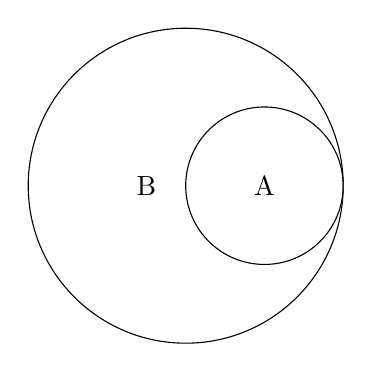
\begin{tikzpicture}
	\draw (0,0) circle (1cm);
	\draw (-1,0) circle (2cm);
	\node at (0,0) {A};
	\node at (-1.5, 0) {B};
\end{tikzpicture}

\ex{}{
	The set of integers with squares less than 100 is not a subset of the set of nonnegative integers
	because -1 is in the former set [as $\left( -1 \right) ^2 < 10$], but not the later set. The set of people who
	have taken discrete mathematics at your school is not a subset of the set of all computer science
	majors at your school if there is at least one student who has taken discrete mathematics who is
	not a computer science major.
}

\thm{}{
	For every set $S$
	\begin{enumerate}
		\item $\O \subseteq S$
		\item $S \subseteq S$
	\end{enumerate}

	\begin{enumerate}
		\item
		      \begin{myproof}
			      We will prove that $\O \subseteq S$, using a vacuous proof \\
			      Let $S$ be a set. \\
			      To show $\O \subseteq S$ we must show that $\forall x \left( x \in \O \to x \in S \right) $ is $T$. \\
			      Because $\O$ contains no elements $x \in  \O$ is always $F$/ \\
			      This follows that the implication $x \in \O \to x \in S$ is always $T$ \\
			      Hence $\O \subseteq S$ \\
		      \end{myproof}

	\end{enumerate}
}

\dfn{Proper subset}{
	A set $A$ is \textit{proper subset} of a set $B$ if and only if every element of $A$ is also an element of $B$ and
	$A \neq B$. Denoted by $A \subset B$. I.e.
	\[
		\exists x \left( x \notin A \wedge x \in B \right) \wedge \forall x \left( x \in A \to x \in B \right)
	\]
	Is $T$.
}

\dfn{Further Equality}{
	Two sets $A$ and $B$ are equal if $A \subseteq B \wedge  B \subseteq A$ is $T$. I.e.
	$A = \left\{ \O, \left\{ a \right\}, \left\{ a \right\}, \left\{ b \right\}, \left\{ a, b \right\}     \right\}  $
	and $B = \left\{ x  \mid x \text{ is a subset of the set } \left\{ a,b \right\}  \right\}  $ are equal.
}

\subsection{Cardinality}

\dfn{Cardinality}{
	The number of distinct elements $n$ in a set $A$. Denoted by $\left| A \right| = n$.
	Where $n$ is a non-negative integer, we say that $A$ is a finite set.
}

\dfn{Infinite set}{
	A set $A$ is infinite if it is not finite. I.e. $\left| A \right| = \infty$
}


\subsection{Power Set}

\dfn{Power Set}{
	A set containing all the subsets of a given set $A$. Denoted by $\mathcal{P} \left( A \right) $. If a set has $n$
	distinct elements, then the cardinality of the power set is $2^{n}$.
}

\ex{}{
	\qs{}{
		What is the power set of the set $ \left\{ 0,1,2 \right\}  $
	}

	\sol{
		\[
			\mathcal{P}(\left\{ 0,1,2 \right\} ) = \left\{ \O, \left\{ 0 \right\}, \left\{ 1 \right\}, \left\{ 2 \right\},,
			\left\{ 0,1 \right\}, \left\{ 0, 2  \right\}, \left\{ 1,2 \right\}, \left\{ 0,1,2 \right\}        \right\}
		\]
	}
}

\ex{}{
	\qs{}{
		What is the power set of $\O$
	}

	\sol{
		\[
			\mathcal{P}(\O) = \left\{ \O \right\}
		\]
	}

	\qs{}{
		What is the power set of $\left\{ \O \right\} $
	}

	\sol{
		\[
			\mathcal{P}\left( \left\{ \O \right\}  \right) = \left\{ \O, \left\{ \O \right\}  \right\}
		\]
	}
}

\subsection{N-Tuples}
\dfn{Ordered N-Tuple}{
	N-tuple $\left( a_1, a_2, \ldots, a_n \right) $ is the ordered collection that has $a_1$ as its first element,
	$a_2$ as its second element, \ldots, and $a_n$ as its $n$th element.
}

Two n-tuples are equal if an only if each corresponding pair of their elements is equal, i.e. $\left( a_1, a_2, \ldots,
	a_n\right) = \left( b_1, b_2, \ldots, b_n \right)  $ are equal if and only if $a_i = b_i$, for $i = 1, 2,\ldots,n$.
\\

Ordered 2-tuples are called \textit{ordered pairs}. The ordered pairs, $\left( a, b \right) $ and $\left( c, d \right) $
are equal if and only if $a = c$ and $b = d$.


\subsection{Cartesian Products}

\dfn{Cartesian Product}{
	Let $A$ and $B$ be sets. The \textit{Cartesian Product} of $A$ and $B$, denoted by $A \times B$, is the set of all
	ordered pairs $\left( a, b \right) $, where $a \in A$ and $b \in B$. I.e.
	\[
		A \times B = \left\{ \left( a, b \right)  \mid a \in A \wedge b \in  B  \right\}
	\]
	The number of items in the Cartesian product of two sets is the product of the cardinality of each set.
}

\ex{}{
	\qs{}{
		What is the Cartesian product of $A = \left\{ 1, 2 \right\} $ and $B = \left\{ a, b, c \right\} $
	}

	\sol{
		\[
			A \times B = \left\{ \left( 1,a \right), \left( 1,b \right), \left( 1,c \right), \left( 2,a  \right),
			\left( 2,b \right), \left( 2, c \right)       \right\}
		\]
	}

	\qs{}{
		Show that the Cartesian product $B \times  A$ is not equal to the Cartesian product $A \times  B$.
	}

	\sol{
		\[
			B \times A = \left\{ \left( a, 1 \right) \left( a, 2 \right), \left( b, 1 \right), \left( b,2 \right), \left(
			c,1 \right), \left( c, 2 \right)       \right\}
		\]
		$\therefore A \times B \neq B \times A$
	}

}

\dfn{Cartesian Product of more than two sets}{
	The Cartesian product of the sets $A_1,A_2,\ldots,A_n$,denoted by $A_1 \times A_2 \times \ldots \times  A_n $,
	is the set of ordered $n$-tuples $\left( a_1,a_2, \ldots,a_n \right) $, where $a_i$ belongs to $A_i$ for $i =
		1,2,\ldots, n$. I.e.
	\[
		A_1\times A_2 \times \ldots \times A_n = \left\{ \left( a_1,a_2,\ldots a_n \right)  \mid a_i \in A_i \text{ for
		}  i = 1,2,\ldots,n  \right\}
	\]
}


\ex{}{
	\qs{}{
		What is the Cartesian product $A \times  B \times C$, where $A = \left\{ 0, 1 \right\} $, $B = \left\{ 1,2 \right\}
		$, $C = \left\{ 0,1,2 \right\} $.
	}

	\sol{
		\[
			A \times B \times C = \left\{ \left( 0,1,0 \right), \left( 0,1,1 \right), \left( 0,1,2 \right), \left( 0,2,0
			\right),  \left( 0,2,1 \right), \left( 0,2,2 \right), \left( 1,1,0 \right), \left( 1,1,1 \right) ,
			\left( 1,1,2\right),   \left( 1,2,0 \right), \left( 1,2,1 \right), \left( 1,2,2 \right)
			\right\}
		\]
	}
}

We use the notation $A^2$ to denote $A \times A$, the Cartesian product of $A$ and itself. Therefore
\[
	A^n = \left\{ \left( a_1, a_2,\ldots,a_n \right)  \mid a_i \in A \text{ for } i = 1,2,\ldots,n  \right\}
\]

\ex{}{
	Suppose $A = \left\{ 1,2 \right\} $. \\
	It follows $A^2 = \left\{ \left( 1,1 \right), \left( 1,2 \right), \left( 2,1
		\right), \left( 2,2 \right)     \right\} $, \\
	and $A^3 = \left\{ \left( 1,1,1 \right), \left( 1,1,2 \right),
		\left( 1,2,1 \right), \left( 1,2,2 \right), \left( 2,1,1 \right), \left( 2,1,2 \right), \left( 2,2,1 \right), \left(
		2,2,2\right)         \right\} $
}

\ex{}{
	\qs{}{
		What are the ordered pairs in the less than or equal to relation, which contains, $\left( a, b \right) $ if $a \leq
			b$, on the set $\left\{ 0,1,2,3 \right\} $
	}

	\sol{
		Let $R$ be the relation on the set $\left\{ 0,1,2,3  \right\} $, if $a \leq b$. \\
		\begin{align*}
			R = \left\{ \left( 0,0 \right), \left( 1,1 \right), \left( 2,2 \right), \left( 3,3 \right), \left( 0,1
			\right),  \left( 0,2 \right), \left( 0,3 \right), \left( 1,2 \right), \left( 1,3 \right), \left( 2,3 \right)            \right\}
		\end{align*}
	}
}

\subsection{Set Notation with Quantifiers}


We can restrict the domain of a quantifier to a set, I.e. Where $S$ is a set $\forall x \in S \left( P \left( x \right)
	\right) $, denotes the universal quantification of $P \left( x \right) $ for all elements in the set $S$. Which is
shorthand for $\forall x \left( x \in S \to P \left( x \right)  \right) $


\ex{}{
	$\forall x \in \mathbb{R} \left( x^2 \geq 0 \right) $ means "the square of any real number is greater than or equal
	to $0$". \\
	$\exists x \in \mathbb{Z} \left( x^2 = 1 \right) $ means "there exists an integer whose square is $1$"
}

\subsection{Truth Sets and Quantifiers}

\dfn{Truth Set}{
	For a predicate $P$ the truth set of $P$ is the set of all elements in the domain of discourse that make $P$ true.
	I.e. let $S$ be a set. The truth set of $P \left( x \right) $ is
	\[
		\left\{ x \in S  \mid  P \left( x \right)  \right\}
	\]
}

\ex{}{
	\qs{}{
		What are the truth set of the predicates $P \left( x \right) $, $Q \left( x \right) $, and $R \left( x \right)
		$, where the domain is the set of integers, and $P \left( x \right)\text{: }  | x | = 1 $, $Q \left( x
			\right)\text{: }
			x^2 = 2$, and $R \left( x \right)\text{: }  | x | = x  $
	}

	\sol{

		\noindent The truth set of $P$ is $\left\{ x \in \mathbb{Z}  \mid  |x| = 1 \right\} $ \\
		The truth set of $Q$ is $\left\{ x \in Z  \mid x^2 = 2 \right\} $ \\
		The truth set of $R$ is $\left\{ x \in \mathbb{Z}  \mid  |x| = x \right\} $
	}
}

\nt {
	$\forall x P \left( x \right) $ is $T$ over the domain $\mathbb{U}$ if and only if the truth set of $P$ is $\mathbb{U}$.
	\\
	$\exists x P \left( x \right) $ is $T$ over the domain $\mathbb{U}$ if and only if the truth set of $P$ is not empty.
}

\chapter{Set Operations}

\section{Set Operations}

\subsection{Union}

\dfn{Union}{
	Let $A$ and $B$ be sets. The \textit{union} of $A$ and $B$, denoted by $A \cup B$, is the set of all elements that
	are either in $A$ or in $B$ or in both. I.e.
	\[
		A \cup B = \left\{ x  \mid  x \in A \vee x \in B \right\}
	\]
}

\subsection{Intersection}

\dfn{Intersection}{
	Let $A$ and $B$ be sets. The \textit{intersection} of $A$ and $B$, denoted by $A \cap B$, is the set of all elements
	that are in both $A$ and $B$. I.e.
	\[
		A \cap B = \left\{ x  \mid  x \in A \wedge x \in B \right\}
	\]
}

\subsection{Complement}

\dfn{Complement}{
	Let $A$ be a set. The \textit{complement} of the set A (with respect to $\mathbb{U}$), denoted by $\overline{A}$ is the set
	$\mathbb{U} - A$. I.e.
	\[
		\overline{A} = \left\{ x \in \mathbb{U}  \mid x \notin A \right\}
	\]
}

\subsection{Difference}

\dfn{Difference}{
	Let $A$ and $B$ be sets.  The \textit{difference} of $A$ and $B$, denoted by $A - B$, is the set of all elements
	that are in $A$ but not in $B$. I.e.
	\[
		A - B = \left\{ x  \mid  x \in A \wedge x \notin B \right\}
	\]
	Or
	\[
		A - B = A \cap \overline{B}
	\]
}

\subsection{Symmetric Difference}

\dfn{Symmetric Difference}{
	Let $A$ and $B$ be sets. The \textit{symmetric difference} of $A$ and $B$, denoted by $A \oplus  B$, is the set
	of all elements that are in exactly one of $A$ and $B$. I.e.
	\[
		A \oplus B = \left( A - B \right) \cup \left( B - A\right)
	\]
}

\ex{}{
	\qs{}{
		\begin{align*}
			\mathbb{U} = \left\{ 0,1,2,3,4,5,6,7,8,9,10 \right\} \\
			A = \left\{ 1,2,3,4,5 \right\}                       \\
			B = \left( 4,5,6,7,8 \right)
		\end{align*}
		What is $A \oplus B$
	}

	\sol{
		\[
			A \oplus B = \left\{ 1,2,3,6,7,8 \right\}
		\]
	}
}

\subsection{The Cardinality of the Union of Two Sets}

The cardinality of the union of two sets $A$ and $B$ is given by
\[
	\left| A \cup B \right| = \left| A \right| + \left| B \right| - \left| A \cap B \right|
\]

\section{Set Identities}

\subsection{Identity Laws}

\begin{align*}
	A \cap   \mathbb{U} = A \\
	A \cup  \O = A
\end{align*}

\subsection{Domination Laws}

\begin{align*}
	A \cup \mathbb{U} = \mathbb{U} \\
	A \cap \O = \O
\end{align*}

\subsection{Idempotent Laws}

\begin{align*}
	A \cup A = A \\
	A \cap A = A
\end{align*}

\subsection{Commutative Laws}

\begin{align*}
	A \cup B = B \cup A \\
	A \cap B = B \cap A
\end{align*}

\subsection{Associative Laws}

\begin{align*}
	A \cup \left( B \cup  C \right)  = \left( A \cup B \right)  \cup C \\
	A \cap \left( B \cap C  \right)  = \left( A \cap B \right)  \cap C
\end{align*}

\subsection{Distributive Laws}

\begin{align*}
	A \cup \left( B \cap C \right)  = \left( A \cup B \right)  \cap \left( A \cup C \right) \\
	A \cap \left( B \cup  \right)  = \left( A \cap B \right)  \cup \left( A \cap C \right)
\end{align*}

\subsection{De Morgan's Laws}
\begin{align*}
	\overline{A \cap  B} = \overline{A} \cup \overline{B} \\
	\overline{A \cup B } = \overline{A} \cap \overline{B}
\end{align*}

\section{Exercises}

\qs{}{
	List the members of these sets
	\begin{enumerate}
		\item  $\left\{ x  \mid x \text{ is a real number such that } x^2 = 1 \right\}$
		\item
		\item
		\item
		\item $ \left\{ x  \mid  x \text{ is an integer such that } x^2 = 2 \right\} $
	\end{enumerate}
}

\sol{
	\begin{enumerate}
		\item $\left\{ -1, 1 \right\} $
		\item
		\item
		\item
		\item $ \O $
	\end{enumerate}
}

\end{document}
